\chapter{Literature Review}
\label{chapter:litRev}
Several researchers have proposed various ideas for implementing an FPGA-based LU solver. These methods vary mainly with the degree of parallelism extracted from the problem and scheduling methods.

In \cite{Kapre} N. Kapre and A. DeHon proposed a method at the International Conference on Field-Programmable Technology in 2009. He accelerated the LU decomposition of sparse matrices on FPGA using a mesh-grid type architecture in NoC. The significant advantage of his approach is that it’s scalable, which is achieved by utilizing the symbolic analysis step of the KLU solver to generate the data flow graph. All the PEs are independent and can make local decisions. This architecture exploits fine-grained parallelism. This particular architecture has obtained a speedup of 1.2-64x using a 250 MHz Xilinx Virtex-5 FPGA compared to the Intel Core i7 965 processor. The mesh architecture and the structure of processing elements is shown in the below figure:-

\begin{figure}[H]
    \centering
    \begin{subfigure}[b]{0.5\textwidth}
        \centering
        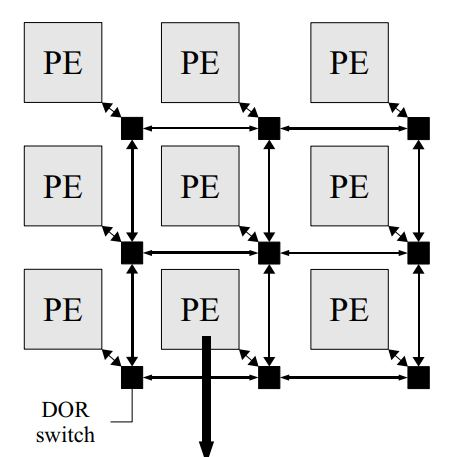
\includegraphics[width = 0.95\linewidth]{./ReviewLit/kapreArch1.JPG}
        \caption{NOC Configuration}
    \end{subfigure}%
    \begin{subfigure}[b]{0.5\textwidth}
        \centering
        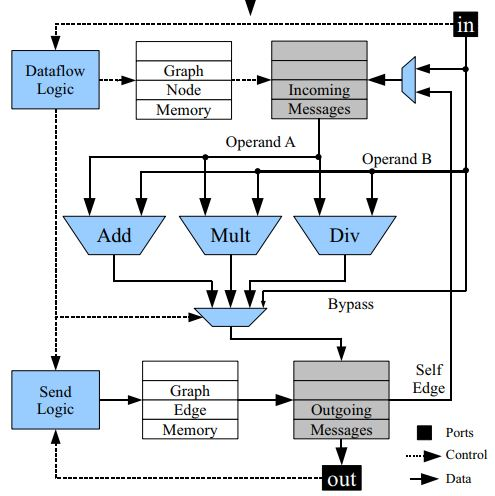
\includegraphics[width = 0.95\linewidth]{./ReviewLit/kapreArch2.JPG}
        \caption{Internal Structure of Processing Element}
    \end{subfigure}
    \caption{NOC based hardware configuration (in \cite{Kapre})}
    \label{fig:Into:kapre}
\end{figure}
In \cite{WuWei}, Wu and Wei have proposed architecture at Reconfigurable Computing: Architectures, Tools, and Applications in 2011 that exploits the coarse-grained parallelism. Each node is connected to an Altera Nios processor attached to a single-precision floating-point unit. Considering coarse-grained parallelism was targeted, the reported speed gain was in the range of 0.5-5.36x, which is not much impressive. Benchmark matrices are smaller and cannot compare results to previous FPGA implementations.
\begin{figure}[H]
    \centering
    \begin{subfigure}[b]{0.5\textwidth}
        \centering
        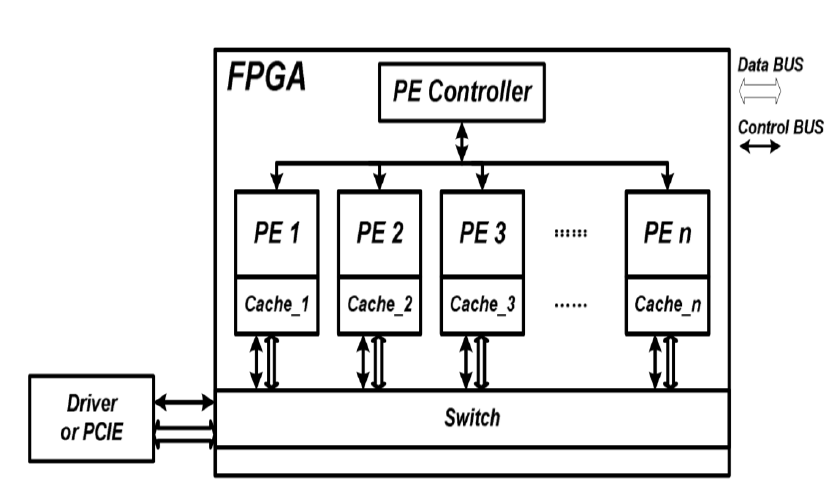
\includegraphics[width = 0.95\linewidth]{./ReviewLit/Wei_FPGA.png}
        \caption{FPGA architecture proposed by Wei}
    \end{subfigure}%
    \begin{subfigure}[b]{0.5\textwidth}
        \centering
        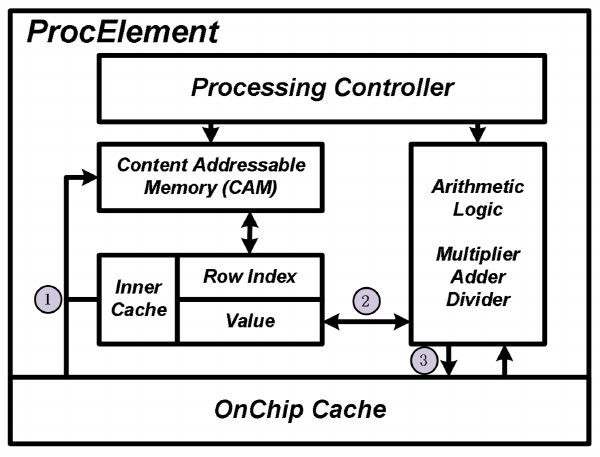
\includegraphics[width = 0.95\linewidth]{./ReviewLit/Wei_PE.png}
        \caption{Internal Structure of Processing Element}
    \end{subfigure}
    \caption{Crossbar switch based hardware configuration (in \cite{WuWei})}
    \label{fig:Into:kapre}
\end{figure}
In \cite{Nechma}, T. Nechma and M. Zwolinski presented an approach at IEEE Transactions on Computers in 2015  to leverage medium-grain parallelism for LU decomposition based on the column-based parallelism using the Gilbert-Peierls Algorithm. The architecture prepares execution schedule sing symbolic analysis. It maps the computation of each column to processing consist of MAC unit, divider unit, and BRAM, and it is scheduled using the ASAP method. The architecture used is shown in the figure below: -
\begin{figure}[H]
    \centering
    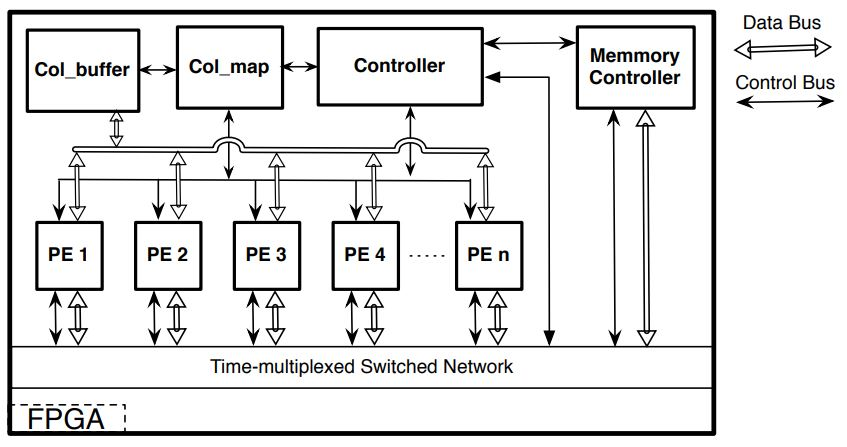
\includegraphics[width = 0.5\linewidth]{./ReviewLit/nechmasArchitecture.JPG}
    \caption{Hardware Architecture used by Nechma \cite{Nechma}}
    \label{fig:Intro:nechma}
\end{figure}
The method used in this report is based on the approach similar to the Nechma's \cite{Nechma}. Our scheduler is geared to leverage the fine-grain parallelism using the set of deeply pipelined processing elements and low latency block RAMs available in FPGAs. 